\documentclass[a4paper]{article}
\let\subsubsubsection\paragraph
\let\subsubsubsubsection\subparagraph
\setcounter{secnumdepth}{4}
\setcounter{tocdepth}{4}
\usepackage[utf8]{inputenc}
\usepackage[T1]{fontenc}
\usepackage[italian]{babel}
\usepackage{graphicx}
\usepackage{lscape}
\usepackage{fancyhdr}
\usepackage{totpages}
\usepackage{enumerate}
\usepackage{float}
\usepackage{color}
\usepackage[pdftex]{hyperref}
\usepackage{listings}
\usepackage{tabularx}
\usepackage{amsthm}
\hypersetup{colorlinks,breaklinks,linkcolor=blue,urlcolor=black}

\usepackage{fancyhdr}
\newcommand{\fncyblank}{\fancyhf{}}
%\newenvironment{abstract}%
%{\fncyblank\null\vfill\begin{center}%
%\bfseries\abstractname\end{center}}%
%{\vfill\null}

\renewcommand{\baselinestretch}{1.25}

\pagestyle{fancy} 

\makeindex

% Definizione di nuovi "tokens" (e valori che possono assumere)
\newtoks\titolo
\newtoks\sottotitolo
\newtoks\filename
\newtoks\data
\newtoks\versione
\newtoks\distribuzione

% Titolo documento + titolo a pie' pagina e data (tokens)
\titolo={F1 Simulator} 
\sottotitolo={Progetto di Sistemi concorrenti e distribuiti} 
\data={12 Settembre 2010}

% Informazioni documento (tokens)
\filename={Relazione.pdf}
\versione={0.3}
\distribuzione={Prof. Vardanega Tullio \\
		     	& Miotto Nicola \\
			& Nesello Lorenzo
}

% Header (left, center, right)
\lhead{} 
\chead{}
\rhead{}
\renewcommand{\headrulewidth}{0.4pt}
% Footer (left, center, right)
\lfoot{} \cfoot{} \rfoot{\thepage/\pageref{TotPages}}
\renewcommand{\footrulewidth}{0.4pt}

% Inizio documento LaTeX
\begin{document} %produce il titolo a partire dai comandi \title, \author e \date

\begin{center}
\vspace*{1,0 cm}
\huge\textbf{\the\titolo} \\ %LARGE != large
\vspace{0,2 cm}
\large\the\sottotitolo \\
\vspace{0,4 cm}
\large\the\data
\end{center}
\begin{center}
\vspace{1,75 cm}

% Sommario
\begin{abstract} 
\begin{center}
Relazione sul progetto di Sistemi Concorrenti e Distribuiti.
\end{center}
\end{abstract}
\vspace{1,50 cm}

% Informazioni documento
\textbf{Informazioni documento} \\ \vspace{0.5cm}
\begin{tabular}{r | l }
\textbf{Nome file}      & \the\filename         \\
\textbf{Versione}       & \the\versione         \\
\textbf{Distribuzione}  & \the\distribuzione    \\ \\
\end{tabular}
\vspace{0,3cm}
\end{center}

\newpage

\tableofcontents
\newpage
\listoffigures
\newpage
%\chapter{Descrizione del progetto}
\section{Progetto}
Il progetto riguarda l'analisi e la risoluzione delle problematiche di progettazione di un simulatore concorrente e distribuito di una competizione sportiva assimilabile a quelle automobilistiche di Formula 1.
Il sistema da simulare dovr� prevedere:
\begin{itemize}
    \item{un circuito selezionabile in fase di configurazione, dotato della pista e della corsia di rifornimento, ciascuna della quali soggette a regole congruenti di accesso, condivisione, tempo di percorrenza, condizioni atmosferiche, ecc.}
    \item{un insieme configurabile di concorrenti, ciascuno con caratteristiche specifiche di prestazione, risorse, strategia di gara, ecc.}
    \item{un sistema di controllo capace di riportare costantemente, consistentemente e separatamente, lo stato della competizione, le migliori prestazioni (sul giro, per sezione di circuito) e anche la situazione di ciascun concorrente rispetto a specifici parametri tecnici}
    \item{una particolare competizione, con specifica configurabile della durata e controllo di terminazione dei concorrenti a fine gara.}
\end{itemize}

\section{Problematiche}
\subsection{Introduzione}
In questo capitolo verranno analizzate le problematiche legate alla realizzazione di un sistema concorrente e distribuito.
\subsection{Enuncazione problematiche}
Nella seguente sezione verranno esposte le problematiche emerse nel corso dell'analisi del sistema da progettare. Tali
problematiche esistono perchè il sistema presenta le seguenti caratteristiche:
\begin{itemize}
\item il sistema è concorrente. Di conseguenza presenterà un numero maggiore di 2 entità attive
che eseguiranno concorrentemente;
\item alcune risorse sono condivise e accedute quindi concorrentemente;
\item il simulatore viene eseguito su un sistema operativo del cui scheduler non sono conosciute le specifiche;
\item il sistema presenta delle componenti distribuite nella rete;
\end{itemize}
\subsection{Gestione del tempo}
Un simulatore di formula 1 racchiude intrinsecamente dei vincoli in termini di coerenza temporale. 
Una competizione è scandita da istanti di tempo: un istante iniziale, uno finale e vari istanti 
intermedi che segnano, per esempio, la fine della lap di un concorrente, oppure il passaggio di un concorrente da un settore
a quello dopo del circuito. Vi sono inoltre vincoli di coerenza temporale dati dai tempi accumulati nel corso
della gara. Questi potrebbero essere il tempo di attraversamento di un tratto come il tempo necessario
a effettuare un giro. I secondi, chiaramente, dipendono dai primi. 
In un sistema simulato è necessario che per più simulazioni regolate dalle stesse condizioni, 
gli intervalli temporali calcolati siano gli stessi. Questo potrebbe risultare problematico dal momento che
lo scheduler non rispetta vincoli di tempo definiti o comunque conosciuti a priori.
\subsection{Sorpassi impossibili}
Una problematica affrontata nel corso dell'analisi del simulatore da progettare
è stata quella relativa ai sorpassi. Come accennato all'inizio
della sezione, non possono essere fatte assunzioni di determinismo sullo scheduler. 
Ipotizzando un sistema in cui ogni concorrente
corrisponda ad un'entità attiva (task) e in cui ogni tratto del circuito sia una risorsa condivisa fra i task a molteplicità
limitata (come è plausibile pensare per un simulatore di F1), è possibile che si verifichino scenari anomali.\\
Per esempio:
\begin{enumerate}
\item un task concorrente dovrebbe, per questioni temporali, iniziare ad attraversare un tratto e ottenere quindi la risorsa;
\item lo scheduler prerilascia il task e assegna un quanto di tempo ad un altro task concorrente che in termini temporali
è dietro. Il task ottiene la risorsa tratto (la stessa del task precedente);
\item il task ottiene altri quanti e attraversa;
\item lo scheduler prerilascia il task corrente e riassegna il processore al vecchio task il quale anche attraversa il tratto.
\end{enumerate}
Non prestando attenzione a possibilità di questo tipo, se il tratto fosse di molteplicità 1 si avrebbe che un concorrente 
appare alla fine del tratto quando, per questioni fisico/temporali, avrebbe dovuto rimanere dietro.
\subsection{Determinismo}
Come definito in \emph{Simulation: The Engine Behind The Virtual World, Roger D. Smith, Chief Scientist, ModelBenders LLC}:

\emph{``Simulation is the process of designing a model of a real or imagined system and
conducting experiments with that model. The purpose of simulation experiments is to
understand the behavior of the system or evaluate strategies for the operation of the system.''}

%\emph{``per simulazione si intende un modello della realtà che consente di valutare e prevedere lo 
%svolgersi dinamico di una serie di eventi o processi susseguenti all'imposizione di certe condizioni da parte dell'analista
%o dell'utente''}.\\
Considerando quindi che la simulazione deve permettere di comprendere il comportamento del sistema, è necessario che il sistema abbia 
un comportamento prevedibile. Ciò non significa che ogni componente di non determinismo sia non desiderata. Il non determinismo
può essere inserito in modo controllato, ovvero consapevoli del contensto e dei momenti in cui esso si possa verificare. Soprattutto,
il nondeterminismo deve rispecchiare un eventuale non determinismo presente anche nel sistema reale e non solo in quello simulato.\\
Il comportamento dello scheduler sottostante il sistema che verrà sviluppato non è prevedibile. Considerando che il non determinismo
introdotto dallo scheduler non è controllabile, si presenta
il problema di riuscire a progettare il simulatore in modo
che il comportamento sia del tutto indipendente dall'architettura del sistema operativo su cui viene eseguito. In questo
modo si potrà avere un sistema la cui correttezza sia verificabile e capace di fornire dati consistenti.
\subsection{Componenti di non determinismo (Lorenzo)}
\label{non_determinismo}
Dopo aver analizzato le problematiche dovute al determinismo del progetto si possono pensare anche ai fattori che diano del non determinismo.
Per non determinismo si intende la possibilit\`{a} di non prevedere precisamente l'andamento della gara a priori. Questa componente pu\`{o} essere non desiderabile per certi aspetti mentre, se gestita, pu\`{o} dare del valore aggiunto alla simulazione. Nel caso di \emph{F1\_Sim} \`{e} desiderabile riuscire a gestire il non determinismo, che da quindi valore aggiunto al progetto.
\subsection{Stalli (Lorenzo)}
\label{stalli}
In un sistema concorrente lo stallo è una delle probelmatiche pi\`{u} importanti da affrontare. Per stallo si intende lo stato in cui nessun processo pu\`{o} pi\`{u} eseguire. Affinch\`{e} si verifichi lo stallo di devono verificare tutte le 4 pre-condizioni ben riconoscibili:
\begin{itemize}
\item {Mutua Esclusione :} assicura che, a ogni instante, non pi\`{u} di un processo abbia possesso di una risorsa (fisica o logica) condivisa.La sequenza di azioni che opera sulla risorsa \`{e} detta sezione critica
\item{Cumulazione di risorse (hold-and-wait) :} i processi possono accumulare risorse e trattenerle mentre attendono di acquisirne altre
\item{Assenza di prerilascio :} le risorse vengono rilasciate solo volontariamente
\item{Attesa Circolare :} un processo attende almeno una risorsa in possesso del successivo processo in catena
\end{itemize}
Nella progettazione e realizzazione del sistema si dovr\`{a} quindi fare attenzione per evitare il verificarsi delle quattro condizioni, impedendo cos\`{i} gli stalli.
\subsection{Realismo fisico}
Il realismo fisico di un simulatore di formula uno è determinato principalmente da due fattori:
\begin{itemize}
\item realismo dato dall'interazione tra ogni concorrente e l'ambiente statico. Ovvero, l'impatto che hanno
le caratteristiche fisiche dell'ambiente circostante quali, ad esempio, forma e caratteristiche della pista;
\item realismo dato dall'interazione tra un concorrente e gli altri concorrenti. Questo tipo di realismo 
dipende quindi da caratteristiche dinamiche dell'ambiente e richiede che le valutazioni dei singoli concorrenti
vengano fatte in rapporto allo stato degli altri concorrenti. Viceversa, le scelte dei singoli concorrenti
devono poter influenzare le scelte degli altri concorrenti.
\end{itemize}
\subsection{Gestione delle istantanee di gara}
Requisito essenziale per poter presentare i dati relativi all'andamento della competizione è riuscire ad ottenere una
snapshot della gara in un determinato istanto. Ovvero, dato un istante di tempo \emph{t} o un evento \emph{e}, bisogna
poter risalire allo stato dei concorrenti e della gara in generale in quel momento. In tal modo sarà reso possibile
monitorare l'evolversi della competizione. Bisogna però tenere in considerazione che qualunque entità provvede allo scatto
dell'istantanea sarà soggetta alle stesse problematiche legate alle altre entità attive dipendenti dallo scheduler. 
Di conseguenza è lecito pensare che uno snapshot possa risultare inconsistente se viene eseguito, per motivi di 
prerilascio, metà ad un istante
\emph{t} e l'altra metà ad un istante \emph{t+f}, ad esempio. La distribuzione aggiunge un ulteriore livello di complessità
al problema, poichè il ritardo potrebbe essere causato non solo dallo scheduler, ma anche dalla rete.
\subsection{Robustezza del sistema distribuito (Lorenzo)}
Progettando un sistema distribuito bisogna tenere in considerazione alcune problematiche che, se ben risolte, portano a un prodotto distribuito robusto.
I punti principali su cui focalizzare l'attenzione sono
\begin{itemize}
\item Apparenza all'utente di un sistema unitario e non l'insieme di pi\`{u} elaboratori
\item Comunicazione fra elaboratori nascosta all'utente
\item Scelta del livello di distribuzione
\item Architettura invariata rispetto al sistema in locale
\end{itemize}
\subsection{Intelligenza artificiale}
Per poter rendere indipendente da controlli esterni l'esecuzione della simulazione, è necessario fornire almeno un accenno
di intelligenza artificiale che riesca a far procedere la gara in modo verosimile. Il problema in questo caso
\subsection{Avvio del sistema}
L'avvio del sistema presenta dei problemi legati alla natura concorrente e distribuita dello stesso.\\
In dettaglio:
\begin{itemize}
\item la natura distribuita introduce il problema della messa in connessione dei nodi. Quando un nodo si connette
è necessario che esso sappia dove sono dislocati gli altri nodi (o almeno quelli necessari) e che gli altri nodi
possano reperire quello appena connesso.
\item la natura concorrente invece introduce dei problemi relativi alla comunicazione delle entità attive. Tali entità
saranno presumibilmente messe in comunicazione o tramite risorse condivise o in modo diretto. Si prospetta quindi la
possibilità che in fase di avvio (essendo l'avvio un processo sequenziale) alcune entità richiedano la connessione con 
altre che non siano ancora pronte o allocate, causando un fault in alcuni casi, in altri un'esecuzione con risultati 
errati.
\end{itemize}
\subsection{Stop del sistema}
Nel caso specifico di un simulatore di formula 1, lo stop deve avvenire innanzitutto a livello logico. Ovvero, deve essere
possibile al sistema poter capire quando la gara è finita in modo da poterlo annunciare.\\
Una volta che la competizione risulti essere completata, le risorse non più necessarie devono essere deallocate e i task
fermati.\\
Quando il sistema viene interrotto definitivamente, non devono più essere presenti server in attesa di connessioni o
thread attivi.
\subsection{Problematiche di distribuzione}
Un sistema che funzioni grazie alla comunicazione remota fra componenti dislocati in diversi nodi nella rete, presenta certamente delle
specifiche problematiche da affrontare. La pi\`{u} critica riguarda di sicuro la robustezza. \`{E} difficile o addiritura utopico sperare
nell'affidabilit\`{a} della rete. La rete presenta sempre dei fault, la cosa importante \`{e} gestirli e non farli propagare in errori. Sicuramente
quindi bisogner\`{a} minimizzare la probabilit\`{a} che un nodo distribuito, perdendo il contatto con il resto del sistema, possa provocare un 
malfunzionamento globale.
'%%%Architettura alto livello%%%
\subsection{Architettura ad alto livello}
Nella seguente sezione verr\`{a} illustrata l'architettura ad alto livello del sistema sviluppato, 
escludendo i dettagli implementativi e legati al linguaggio.
% Componenti del sistema
\subsubsection{Componenti di sistema}
Le principali componenti del sistema sono:
\begin{description}
\item{Competition}
La \emph{Competition} \`{e} l'unit\`{a} atta ad orchestrare l'avvio e la conclusione della corsa. Tale componente, dunque, \`{e} stata concepita per 
offrire le seguenti funzionalit\`{a}:
\begin{itemize}
\item Configurazione parametri di gara:
	\begin{itemize}
		\item numero di giri;
		\item numero di concorrenti;
		\item circuito;
	\end{itemize}
\item Gestione della sessione di iscrizione e accettazione concorrenti (configurati a livello della componente \emph{Box})
\item Avvio delle componenti necessarie al monitoraggio della gara (quali ad esempio \emph{Monitor})
\item Avvio controllato della competizione vera e propria nel momento in cui tutti i prerequisiti di inizio sono soddisfatti, ovvero:
\begin{itemize}
\item la competizione \`{e} stata configurata correttamente;
\item le componenti di controllo e gestione della competizione sono attive e in attesa di comandi;
\item i concorrenti sono stati correttamente registrati alla competizione e in attesa di partire;
\end{itemize}
\end{itemize}
\item{Competitor}
Il \emph{Competitor} \`{e} l'entit\`{a} pensata ad svolgere la gara. \`{E} caratterizzato dalle seguenti sotto-componenti:
\begin{itemize}
\item \textbf{Auto}, ovvero tutte le caratteristiche fisiche legate all'auto, ovvero:
	\begin{itemize}
		\item motore;
		\item capacit\`{a} del serbatoio;
		\item massima accelerazione;
		\item massima velocit\`{a};
		\item gomme montate (mescola, modello, tipo);
		\item livello usura gomme;
		\item livello della benzina nel serbatoio;
	\end{itemize}
\item \textbf{Guidatore}, cio\`{e} le informazioni che descrivono pi\`{u} dettagliatamente il concorrente in gara:
	\begin{itemize}
		\item nome e cognome pilota;
		\item nome scuderia
	\end{itemize}
\item \textbf{Strategia}, ovvero la strategia che sta adottando il pilota, suggerita dai box e dinamica nel corso della gara:
	\begin{itemize}
		\item style di guida, variabile tra conservativo, normale, aggressivo, a seconda dello stato della macchina e delle
			previsioni fatte dai box
		\item numero di lap prima del pit stop
		\item addizionalmente, quando viene fatto un pit stop, la strategia determina anche quali siano le nuove gomme da montare,
		 	la quantit\`{a} di benzina da avere nel serbatoio e il tempo impiegato per il pit stop.
	\end{itemize}
\end{itemize}
Tutte queste informazioni insieme creano quello che viene definito il concorrente di gara. 
Tali informazioni verranno poi usate nel corso della gara per:
	\begin{itemize}
		\item scegliere al momento giusto la miglior traiettoria da seguire, in base alla presenza o meno di altri concorrenti
			nelle vicinanze e alla difficolt\`{a} del tratto;
		\item fornire costantemente aggiornamenti sul suo stato (tramite una parte del modulo \emph{Stats}, informando il computer di bordo
			riguardo a:
			\begin{itemize}
				\item livello di usura gomme;
				\item livello di benzina;
				\item checkpoint attraversato con tempo di arrivo;
				\item insieme al checkpoint verranno aggiornate le informazioni relative a settore e lap;
				\item velocit\`{a} massima raggiunta.
			\end{itemize}
		\item contattare ad ogni giro il box per ottenere una strategia aggiornata;
		\item se suggerito dai box, effettuare un pitstop;
		\item ritirarsi dalla gara una volta che le condizione dell'auto non permettano di poter correre ulteriormente;
		\item banalmente, continuare a correre fino alla fine delle lap prestabilite, dopodich\`{e} fermarsi.
	\end{itemize}
\item{Circuit}
Il circuito è una risorsa finalizzata ad offrire il piano su cui svolgere la competizione. \`{E} condivisa fra tutti i concorrenti in gara e
offre un insieme di funzionalità per poter conoscere le caratteristiche dei vari tratti della pista (compresi i concorrenti presenti
al momento dell'attraversamento). \`{E} composto dalle seguenti sottocomponenti:
\begin{itemize}
\item \textbf{Checkpoint}
\item \textbf{Path}
\item \textbf{}
\end{itemize}
\item{Stats}
\item{Box}
\item{Radio}
\item{Monitor}
\end{description}
 - lista delle componenti con descrizione ad alto livello del loro scopo
 - se necessario fornire un diagramma delle componenti
% Interazione fra le componenti
\subsubsection{Interazione fra le componenti}
 - descrivere ad alto livello l'interazione fra componenti e se necessario aiutarsi con OCR cards
% Strategia adottata per la correttezza temporale
\subsubsection{Strategia adottata per la correttezza temporale}
% Dimostrazione dell'assenza di stallo
\subsubsection{Assenza di stallo}
%%% Architettura in dettaglio %%
\subsection{Architettura in dettaglio}
% Elenco dei task con descrizione
\subsubsection{Risorse attive}
% Elenco risorse condivise con descrizione
\subsubsection{Risorse passive}
\begin{itemize}
\item{Risorse protette}
\item{Altre risorse}
\end{itemize}
%"Analisi della concorrenza"
\subsubsection{Analisi della concorrenza}
	%. analisi dell'interazione risorse e task (senza menzionare la distribuzione)
	%. dimostrazione assenza di racecondition
	%. dimostrazione assenza di starvation
\begin{itemize}
\item{Interazione tra risorse condivise e task}
\item{Assenza di racecondition}
\item{Assenza di starvation}
\end{itemize}
%"Distribuzione"
\subsubsection{Distribuzione}
	%. Elenco risorse distribuite
	%. Interazione risorse distribuite
	%. Misure di fault tolerance
\begin{itemize}
\item{Componenti distribuite}%Con motivazione
\item{Interazione fra le componenti distribuite}
\item{Misure di fault tolerance}
\end{itemize}
% Inizializzazione gara
\subsection{Inizializzazione competizione}
% Stop gara
\subsection{Stop competizione}

%\section{Competizione}
%\section{Circuito}
%\section{Pista}
%\section{Box}
%\section{Tratto}
%\section{Traiettoria}
%\section{Concorrente}
%\section{Sistema di controllo}
%\section{Interfaccia di monitoraggio}
\section{Analisi del supporto tecnologico}
% Scelta dei linguaggi 
	% Ada 
	% Java
	% Bash per l'avvio
% Scelta tecnologiche per la distribuzione
% Scelta del middleware

%\chapter{Bibliografia}
\appendix
\section{Glossario}
\begin{list}{}
\item \textbf{A}\\
\textsc{Antenna}: a receiver put on the toll lane -check-in -check-out that read the the information of a toll tag to recognize a customer and notify the lane controller of his arrival.\\
\item \textbf{B}\\
\textsc{Bank}: a generic bank that represents the entity intended to handle the toll lane customers' account when the toll lane system perform a transaction.\\
\textsc{Barrier}: a physical obstacle positioned on each check-in and check-out. It is intended to prevent an unauthorized customer to pass through.\\
\item \textbf{C}\\
\textsc{Concorrente}: l'entità costituita da pilota e auto che partecipa alla gara correndo sul circuito.\\
\textsc{Cashier (review)}: employee who works in every toll lane station check-in whose task can be summurized in the lsit below:
\begin{itemize}
	\item receive a customer who wants to pass through the toll lane;
	\item calculate the price based on the vehicle type;
	\item take right amount the money and eventually register the customer;
\end{itemize}
\textsc{Card reader}: the device used to read the customer's credit card and perform the transaction with a bank.\\
\textsc{Check-in}: the entering point of the toll lane. There are two kind of Check-in:
\begin{itemize}
\item Express, where a customer che pass through using a toll tag;
\item Normal, where a customer has to stop and pay (using cash or credit card) before being able to pass.
\end{itemize}
Each Check-in has a barrier.\\
\textsc{Check-out}: the exit point of the toll lane. there are two kind of Check-out:
\begin{itemize}
\item Express, where a customer can pass through using a toll tag;
\item Normal, where a customer has to stop and has his ticket validated by the ticket reader before being abel to pass.
\end{itemize}
Each Check-out has a barrier.\\
\textsc{Customer}: the client of the toll lane.\\
\item \textbf{D}
\item \textbf{E}
\textsc{Enterprise server}:\\
\item \textbf{F}
\item \textbf{G}
\item \textbf{H}
\item \textbf{I}
\item \textbf{J}
\item \textbf{K}
\item \textbf{L}\\
\textsc{Lane Controller}: a software system conceived to offer a communication bridge between the input interfaces of the system (like the touchscreen, the ticket reader ...) and the other components (like the station server, the printer ...).\\
\item \textbf{M}
\item \textbf{N}
\item \textbf{O}
\item \textbf{P}\\
\textsc{Printer}: a physical device used by check-in employee to print tickets.\\
\item \textbf{Q}
\item \textbf{R}
\item \textbf{S}\\
\textsc{Station Server}: a server offering the following services:
\begin{itemize}
\item register the toll lane system customer's activities (through the communication with lane controller);
\item store the information about the current prices for the toll lane system service;
\item provide the enterprise server with all the information concerning the toll lane station activities.
\end{itemize}
\item \textbf{T}\\
\textsc{Ticket}: it's sold to the customer at the toll lane station or in a specialised center. It gives the customer the possibility to use the toll lane. It's used at the check-out to leave the toll lane.\\
\textsc{Ticket reader}: physical device used to recognize a valid ticket and eventually notify the lane controller.\\
\textsc{Toll tag}: a device with an RFID chip used by the customer to pass through the express check-in (and check-out) once readed by the antenna.\\
\textsc{Touchscreen}: the physical interface used by the cashier to execute his activities.\\
\item \textbf{U}
\item \textbf{V}
\item \textbf{X}
\item \textbf{Y}
\item \textbf{W}
\item \textbf{Z}
\end{list}

\section{Manuale utente}
\subsection{Prerequisiti}
Il programma pu\`{o} essere eseguito solo su macchine Unix-like. Inoltre, per la compilazione,
\`{e} necessario disporre delle seguenti componenti:
\begin{itemize}
\item gnatmake 4.4.3
\item gcc 4.4.3
\item librerie \textbf{XmlAda 3.2w} installate con comando \underline{xmlada-config} eseguibile anche senza privilegi di root.\\
In caso contrario, scaricare il pacchetto XMLAda da\\
\url{http://libre.adacore.com/libre/download2/}\\
e, dopo la decompressione, seguire le istruzioni incluse per la compilazione ed installazione.
\item librerie \textbf{PolyORB GPL 2009-20090519 (rev. 144248)} installate con comando \underline{polyorb-config} eseguibile anche 
senza privilegi di root\\
In caso contrario, scaricare il pacchetto PolyORB da\\
\url{http://libre.adacore.com/libre/download2/}\\
e, dopo la decompressione, seguire le istruzioni incluse per la compilazione ed installazione.
\end{itemize}
La versione indicata delle librerie \`{e} quella usata per i test. Non si esclude tuttavia che il programma possa funzionare anche con versioni
appena precedenti o successive.
\subsection{Installazione}
Dalla directory radice, eseguire i seguenti comandi:
\begin{itemize}
\item \emph{make competition}\\
per compilare la componente destinata a ospitare la competizione
\item \emph{make box}\\
per compilare la componente destinata a eseguire il box
\item \emph{make tv}
per compilare la componente che verr\`{a} usata per la TV
\end{itemize}
Le tre componenti hanno make diversi perch\`{e} possono essere compilate ed eseguite su macchine separate, comunicando remotamente.
\subsection{Avvio}
Come per la compilazione, dalla directory radice eseguire il comando desiderato fra i seguenti:
\begin{itemize}
\item \emph{./start\_competition.sh}\\
avvier\`{a} la competizione. Apparir\`{a} il pannello di configurazione (del quale verranno forniti dettagli in seguito)
\item \emph{./start\_box.sh n}\\
avvier\`{a} un numero n box. Per eseguire un test in locale \`{e} possibile avviare tanti box quanti quelli stabiliti durante la configurazione
della competizione. In tal caso, l'interfaccia di configurazione dei box presenter\`{a} nello spazio riservato al corbaloc per la connessione
alla competizione, il corbaloc della competizione caricato dal contesto locale. Se invece si volessero avviare i box in altri nodi, il corbaloc
per la registrazione pu\`{o} essere trovato in \\
\emph{competition\_registrationhandler\_corbaLoc.txt}\\
a competi<ione configurata. 
\item \emph{./start\_tv.sh}\\
inizializza una tv. Anche in questo caso, se il corbaloc della competizione \`{e} presente in locale, verr\`{a} impostato di default nel textbox
dedicato. \`{E} comunque possibile reimpostarlo utilizzando il corbaloc salvato nel file\\
\emph{competition\_monitor\_corbaLoc.txt}\\
a competizione configurata.
\end{itemize}
L'interfaccia TV \`{e} possibile copiarla senza necessit\`{a} di ricompilazione in tutte le macchine ove la si voglia eseguire. E' sufficiente,
una volta compilata, copiare il file \emph{start\_tv.sh} e la directory \emph{obj/java/GUI} (mantenendo la gerarchia intatta) in un qualunque
nodo distribuito ed eseguire lo starter.
\subsection{Terminazione}
Per terminare il programma (box, competizione o tv che sia) premere il tasto ``x'' in alto a destra sulla finestra.
\subsection{Interfaccia box}
Nella prima schermata che appare si può selezionare un file di configurazione da cui caricare i dati per i concorrenti. Se non si seleziona l'opzione si passa alla seconda schermata dove si possono impostare a mano, partendo dai valori di default. 
I parametri impostabili sono:
\begin{enumerate}
\item Impostare il nome del concorrente
\item Impostare il cognome del concorrente
\item Impostare la scuderia del concorrente
\item Impostare il livello di seriet\`{a} del box (come descritto da \ref{box})
\item Impostare la massima capacit\`{a} del serbatoio
\item Impostare il livello di benzina iniziale
\item Impostare la mescola delle gomme montate (le gomme a mescola morbida si consumano pi\`{u} rapidamente)
\item Impostare lo stile di guida del concorrente 
\item Impostare la massima accelerazione della macchina
\item Impostare la massima velocit\`{a} raggiungibile
\item Inserire il corbaloc che fa riferimento al Registration Hanlder
\item Pulsante per avviare la competizione
\item Pulsante per riportare la gui allo stato iniziale
\end{enumerate}
\begin{center}
\begin{figure}[H]
	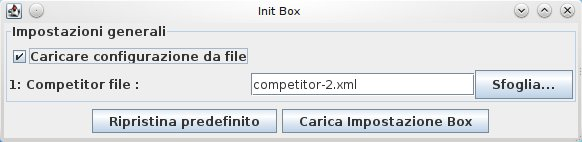
\includegraphics[scale=0.75]{screenshotRelazione/box1.jpeg}
	\caption{Finestra di pre - configurazione del box e del concorrente}
\end{figure}
\end{center}
\begin{center}
\begin{figure}[H]
	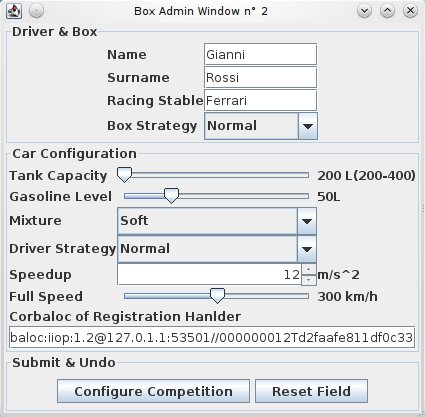
\includegraphics[scale=0.75]{screenshotRelazione/box2.jpeg}
	\caption{Finestra di  configurazione del box e del concorrente}
\end{figure}
\end{center}
Una volta inseriti i dati e premuto il pulsante di avvio della competizione comparir\`{a} una finestra con al suo interno 
\begin{enumerate}
\item Pannello dei consumi medi del concorrente con dati relativi alla benzina (in litri al kilometro) e dell'usura delle gomme (in percentuale relativo a 1 km)
\item Pannello con il log della gara aggiornato a ogni fine settore con dati di tempo di gara, livello di benzina e usura delle gomme
\item Pannello con altre informazioni statiche sulla gara (configurazione iniziale, stile di guida)
\item Pulsante per forzare il pitstop
\end{enumerate}
\begin{center}
\begin{figure}[H]
	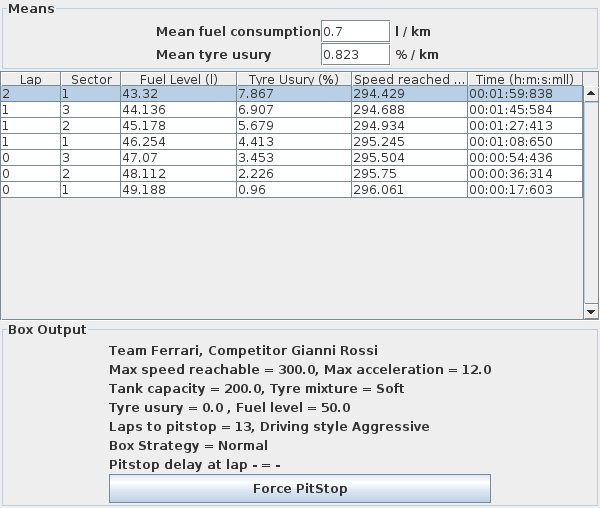
\includegraphics[scale=0.75]{screenshotRelazione/box3.jpeg}
	\caption{Monitor dei box}
\end{figure}
\end{center}
\subsection{Interfaccia competizione}
La prima interfaccia relativa alla competizione serve per impostare la competizione stessa. I parametri da settare sono:
\begin{enumerate}
\item File xml con il tracciato\\
il formato per il file xml del tracciato \`{e} il seguente:
\begin{lstlisting}
<racetrack>
  <sector>
      <checkpoint>
	<length>19.00</length>
	  <mult>7</mult>
	  <angle>140.00</angle>
	  <grip>7.0</grip>
      </checkpoint>
      <!-- altri checkpoint-->
  </sector>
  <!--altri 3 sector strutturati allo stesso modo-->
</racetrack>
\end{lstlisting}
Il checkpoint pu\`{o} avere uno dei seguenti attributi:
\begin{itemize}
\item \textbf{goal=``true''}: obbligatorio in massimo 1 checkpoint. Indica il checkpoint di partenza.
\item \textbf{prebox=``true''}: obbligatorio in massimo 1 checkpoint nel settore 3.
\item \textbf{exitbox=``true''}: obbligatorio in massimo 1 checkpoint nel settore 1.
\end{itemize}
\item Numero di concorrenti richiesti
\item Numero di giri previsti
\item Nome del tracciato
\end{enumerate}
Una volta settati i parameteri e schiacciato il pulsante \emph{Start Competition} verr\`{a} avviato una tv che presenta le informazioni sulle iscrizioni nella parte bassa della finestra. Ogni volta che un concorrente si iscrive compare nella gui e una volta raggiunto il numero di concorrenti stabiliti la gara si avvia e la gui comincia ad offrire i dati disponibili, come spiegato nel paragrafo \ref{interfacciaTv}
\begin{center}
\begin{figure}[H]
	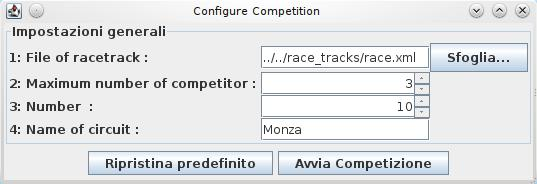
\includegraphics[scale=0.75]{img/ScreenshotRelazione/configureCompetition.jpg}
	\caption{Finestra di configurazione della competizione}
\end{figure}
\end{center}
\subsection{Interfaccia TV}
\label{interfacciaTv}
L'interfaccia della tv consiste in un pannello iniziale con al suo interno un cronometro che scandisce il tempo di aggiornamento delle informazioni seguito da un pannello con le informazioni sul miglior giro e sui migliori tempi nei settori.
L'intervallo per il tempo che scorre \`{e} impostabile se si tratta di una tv configurata tramite il \emph{TvConfigurationWindow}, prestabilito (e molto basso) se si tratta della tv avviata dalla competizione. Il formato della stringa di refresh dev'essere \emph{secondi . millisecondi}.
Questo tempo che scorre \`{e} tempo relativo alla competizione e quindi solidale con il resto del sistema.
Il pannello centrale offre la visualizzazione di due tabelle. La tabella a destra si riferisce all'ultima classifica disponibile mentre a sinistra viene visualizzata la classifica del giro precedente (escluso al primo giro di gara dove viene presentata una tabella vuota).
Nella parte bassa della finestra viene presentato un log della competizione rappresentando a ogni istante di tempo posizione nella pista, numero di checkpoint, numero di settore e giro per ogni concorrente.
\begin{center}
\begin{figure}[h]
	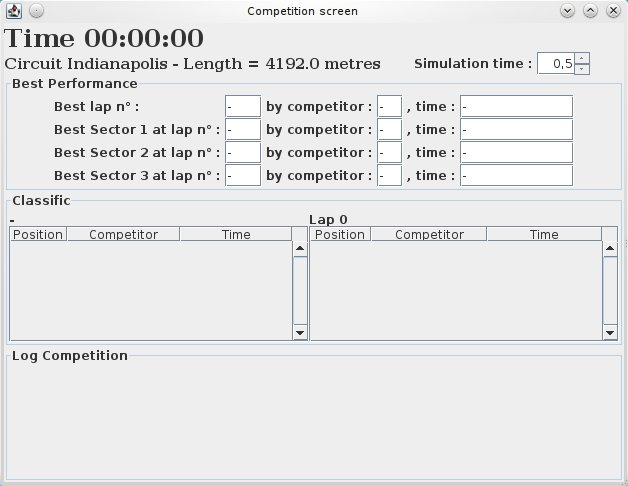
\includegraphics[scale=0.75]{screenshotRelazione/competition2.jpeg}
	\caption{Finestra di visualizzazione dell'andamento della gara}
\end{figure}
\end{center}
\begin{center}
\begin{figure}[h]
	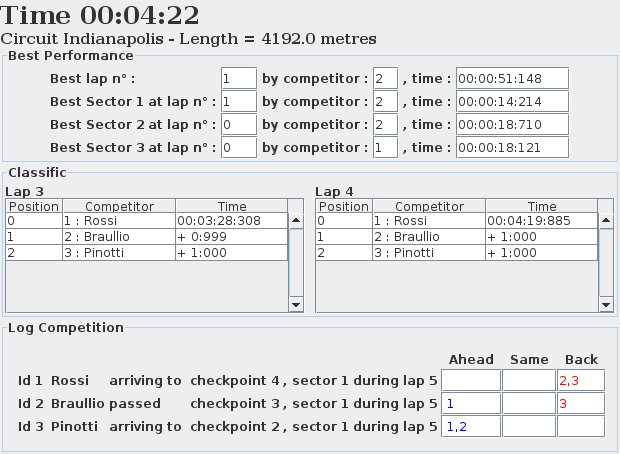
\includegraphics[scale=0.75]{screenshotRelazione/tv2.jpeg}
	\caption{Finestra di visualizzazione dell'andamento della gara - durante la simulazione}
\end{figure}
\end{center}
La componente di avvio dell'interfaccia TV pu\`{o} essere l'interfaccia di competizione oppure una schermata di configurazione dove va inserito il corbaloc del Monitor della competizione e impostato il tempo di refresh per il reperimento delle informazioni. Il pulsante (presente solo nel monitor della competizione) presente in alto a destra permette di modificare il tempo della simulazione.
Nel pannello con il log della competizione sono presenti tre campi per ogni concorrente che rappresentano rispettivamente i concorrenti davanti a lui, nello stesso tratto e dopo di lui.
\begin{center}
\begin{figure}[H]
	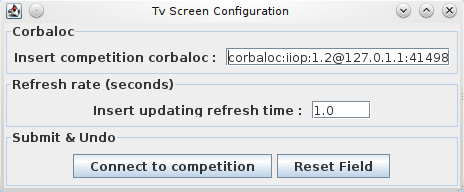
\includegraphics[scale=0.75]{img/ScreenshotRelazione/configurationScreen.jpg}
	\caption{Finestra di configurazione della tv}
\end{figure}
\end{center}

\end{document}
